\documentclass[12pt, a4paper, oneside]{report} 

\usepackage[utf8]{inputenc}   
\usepackage{tabularx}  
\usepackage{amsmath, amssymb}     
\usepackage{graphicx}
\usepackage{float}             
\usepackage{booktabs, array}    
\usepackage{geometry}          
\geometry{top=1in, bottom=1in, left=1.2in, right=1in} 
\usepackage{setspace}            
\onehalfspacing                  
\usepackage{hyperref}             
\hypersetup{colorlinks=true, linkcolor=blue, citecolor=green, filecolor=magenta, urlcolor=cyan}

% --- معلومات المقترح البحثي (Title Page Info) ---
\title{\textbf{Proposed Adaptive Model for Health Data Security in Yemen Based on HIPAA Technical Standards}}
\author{Anwar Hasan Yahya Abohadi}
\date{2026}


\begin{document}
	
	\begin{titlepage}
		\begin{center}
			\vspace*{4.5cm}
			
			{\Large \bf Proposed Adaptive Model for Health Data Security in Yemen Based on HIPAA Technical Standards: A Vision in Cyber Risk Management} \\
			\vspace{2cm}
			
			{\large By:} \\
			{\large \textbf{Anwar Hasan Yahya Abohadi}} \\
			\vspace{2cm}
			
			{\large A Research Proposal Submitted in Partial Fulfillment of the Requirements for the Course: Research Methodology \\ Master Degree in Information Systems} \\
			\vspace{2.5cm}
			
			{\large June 2026}
		\end{center}
	\end{titlepage}
	
	\pagenumbering{roman}
	
	\begin{abstract}
		The rapid global advancement in digital health technologies promises to revolutionize healthcare delivery, yet it introduces severe cybersecurity challenges in fragile and resource-constrained regions. This study addresses the critical security gaps within the Yemeni healthcare sector, where ongoing conflict, fragmented infrastructure, and the absence of a unified national cybersecurity framework leave Electronic Protected Health Information (ePHI) highly vulnerable to cyber threats. To bridge the gap between rigorous global standards and local operational realities, this research proposes a context-specific, adaptive health data security model. By integrating the Technical Safeguards of the Health Insurance Portability and Accountability Act (HIPAA) with the core functions of the National Institute of Standards and Technology (NIST) Cybersecurity Framework (CSF), the model provides a flexible, tiered approach. Built upon three core pillars—an Adaptive Access Control Layer, a Resilient Encryption Layer, and a Lightweight Auditing Layer—the framework leverages open-source solutions (e.g., Keycloak, ELK Stack) and existing local biometric infrastructure to minimize financial and performance overhead on legacy hardware. This conceptual framework offers a pragmatic roadmap for healthcare institutions and policymakers to safeguard patient privacy, improve cyber resilience, and maintain critical healthcare delivery in fragile environments. \\
		\noindent  \textbf{Keywords:}
		Health Data Security, HIPAA, Yemen, Cyber Risk Management, Adaptive Model, NIST CSF.
	\end{abstract}
	\newpage
	
	
	\tableofcontents   
	\listoffigures    
	\listoftables     
	\newpage
	
	
	\pagenumbering{arabic} 
	
	
	\chapter{Introduction} 
	The rapid global advancement in digital health technologies, including Electronic Health Records (EHRs) and telemedicine, promises to revolutionize healthcare delivery by enhancing efficiency, accessibility, and quality of patient care. However, this digital transformation also introduces significant cybersecurity challenges, particularly in regions characterized by fragile infrastructure, political instability, and limited resources \cite{alhammadi2024advancing}, \cite{al2025political}. In such environments, the protection of Electronic Protected Health Information (ePHI) becomes a critical concern, as vulnerabilities can lead to severe consequences, including data breaches, loss of patient trust, and compromised patient safety.
	Yemen, a country currently experiencing prolonged conflict and humanitarian crises, is an example of a challenging context for digital health initiatives. Although the current situation is difficult, the Yemeni health sector is gradually undergoing a digital transformation, with a growing utilization of EHRs and other digital systems \cite{alhammadi2024advancing}. While this transition offers benefits, it also exposes sensitive health data to a wide range of cyber threats, from ransomware attacks to advanced data breaches \cite{abdulrab2021assessing}. These vulnerabilities are compounded by the absence of comprehensive national cybersecurity frameworks and the infancy of cyber risk management practices in many Yemeni institutions \cite{al2023information}. Therefore, there is a dire need for strong but flexible health data security measures that can be effective in the given context of a fragile state.
	
	\section{Problem Statement} 
	The increasing reliance on digital health systems in Yemen, driven by the global trend towards healthcare digitalization, has created a critical disparity between the volume of sensitive ePHI being generated and processed, and the capacity of existing cybersecurity infrastructures to protect it. The current state is characterized by a fragmented approach to health data security, often lacking a unified national strategy or adequately enforced policies \cite{alhammadi2024advancing}, \cite{al2025political}. This leads to several pressing issues:
	\begin{itemize}
		\item{	\textbf{Vulnerability to Cyber Threats:} Yemeni healthcare institutions are highly susceptible to various cyberattacks due to outdated infrastructure, lack of security awareness among staff, and insufficient financial investment in cybersecurity technologies \cite{abdulrab2021assessing}, \cite{al2023information}. This vulnerability directly threatens the confidentiality, integrity, and availability of ePHI.}
		\item{\textbf{Absence of Adapted Frameworkss:} While international standards like the Health Insurance Portability and Accountability Act (HIPAA) in the United States and the National Institute of Standards and Technology (NIST) Cybersecurity Framework (CSF) provide comprehensive guidelines for health data security, their direct and unadapted application in resource-constrained and conflict-affected settings like Yemen is often impractical and unsustainable \cite{nist2024sp80066r2}. There is a significant research gap in developing context-specific, adaptive cybersecurity models that bridge the requirements of global standards with local realities.}
		\item{\textbf{Negative Impact on Healthcare Delivery:} The failure to secure ePHI can result in severe operational disruptions, financial losses, erosion of patient trust, and, most critically, compromised patient safety and privacy \cite{melaku2023context}. These negative impacts further strain an already overburdened healthcare system, hindering efforts towards recovery and development.}
	\end{itemize}
	Therefore, the core problem addressed by this research is the critical gap between the imperative to protect ePHI in the digitalizing Yemeni health sector and the current inability to effectively implement robust, globally recognized cybersecurity standards due to the unique socio-economic, political, and technological constraints of a fragile state.
	
	\section{Purpose Statement} 
	The purpose of this study is to develop and propose an adaptive model for health data security in Yemeni hospitals, based on the technical safeguards of the Health Insurance Portability and Accountability Act (HIPAA) and the principles of the National Institute of Standards and Technology (NIST) Cybersecurity Framework, to effectively mitigate cyber risks in resource-constrained and fragile environments.
	
	\section{Research Questions}
	This study aims to answer the following research questions:
	\begin{itemize}
		\item \textbf{Main Research Question:} How can the technical safeguards of HIPAA and the NIST Cybersecurity Framework be adaptively implemented to enhance health data security in resource-constrained Yemeni hospitals?
		\item \textbf{Sub-Research Questions:}
		\begin{itemize}
			\item[-] What are the primary cybersecurity challenges and vulnerabilities specifically impacting health data protection in Yemeni healthcare institutions?
			\item[-] What are the key components and architectural considerations for an adaptive health data security model that integrates HIPAA technical safeguards and NIST CSF principles, tailored for the unique socio-technical context of Yemen?
			\item [-] What are the expected outcomes, benefits, and potential challenges of implementing such an adaptive model on health data protection and cyber risk management in Yemeni healthcare institutions?
		\end{itemize}
	\end{itemize}
	
	\section{Research Objectives}
	In alignment with the research questions, the objectives of this study are:
	\begin{itemize}
		\item \textbf{General Objective:}To enhance the overall health data security posture in Yemeni hospitals through the development and proposal of a context-specific adaptive cybersecurity model.
		\item \textbf{Specific Objectives:}
		\begin{itemize}
			\item [-] To identify and comprehensively analyze the specific cybersecurity challenges, threats, and vulnerabilities prevalent in the Yemeni healthcare sector, particularly concerning ePHI protection.
			\item [-] To design a pragmatic and adaptive health data security model by integrating the essential technical safeguards of HIPAA and the core functions of the NIST Cybersecurity Framework, ensuring its suitability for resource-constrained and fragile environments.
			\item [-] To evaluate the potential impact, benefits, and feasibility of the proposed adaptive model in improving health data protection, cyber risk management, and compliance within Yemeni healthcare institutions.
		\end{itemize}
	\end{itemize}
	
	\section{Significance of the Study}
	This study holds significant theoretical and practical implications, contributing to both academic knowledge and real-world application in a critical domain.
		\begin{itemize}
		\item \textbf{Theoretical Significance:}
			\begin{itemize}
				\item[-]\textbf{ Contribution to Cybersecurity Literature in Fragile States:}This research contributes to the nascent body of literature on cybersecurity and digital health in fragile and conflict-affected states. It provides a unique perspective on adapting global cybersecurity frameworks (HIPAA, NIST CSF) to environments with severe resource limitations and complex socio-political dynamics, offering insights into the challenges and strategies for effective implementation \cite{nist2024sp80066r2}.
				\item [-]\textbf{ Framework Adaptation Methodology:}The study proposes a methodology for adapting established international cybersecurity standards to local contexts, which can serve as a blueprint for similar efforts in other developing or fragile nations facing comparable challenges in digital health adoption.
			\end{itemize}
		\item \textbf{Practical Significance:}
			\begin{itemize}
				\item [-] \textbf{ Enhanced Health Data Protection:}The primary practical benefit is the provision of a tailored, implementable model that can significantly improve the protection of ePHI in Yemeni hospitals, thereby safeguarding patient privacy and maintaining the integrity and availability of critical health information \cite{hhs2024hipaa}.
				\item [-] \textbf{ Guidance for Policy Makers:}The findings and proposed model offer concrete recommendations for the Yemeni Ministry of Health and other relevant governmental bodies to develop national policies and regulations that are both aligned with international best practices and feasible within the local context \cite{hasegawa2024cybersecurity}, \cite{saad2025fuzzy}.
				\item [-] \textbf{Improved Cyber Risk Management:} By identifying specific vulnerabilities and proposing adaptive safeguards, the study enables Yemeni healthcare institutions to better manage cyber risks, reduce the likelihood of data breaches, and enhance their overall cyber resilience \cite{al2023information}, \cite{melaku2023context}.
				\item [-] \textbf{ Resource-Conscious Solutions:} The emphasis on adaptability and the use of open-source technologies ensures that the proposed solutions are economically viable and sustainable for institutions with limited financial and technical resources \cite{hasegawa2024cybersecurity}, \cite{saad2025fuzzy}.
			\end{itemize}
	\end{itemize}
	\section{Scope and Delimitations}
	This study is specifically delimited to the development and proposal of an adaptive model for health data security within Yemeni hospitals. The focus is primarily on the technical safeguards as outlined by HIPAA, integrated with the core functions of the NIST Cybersecurity Framework (Identify, Protect, Detect, Respond, Recover) \cite{hhs2024hipaa}, \cite{rahmany2026aida}. \\
	\textbf{Scope:}
	\begin{itemize}
		\item The geographical scope is limited to healthcare institutions operating within Yemen.
		\item The study concentrates on the protection of Electronic Protected Health Information (ePHI).
		\item The analysis and proposed model are centered on the technical aspects of cybersecurity, drawing from HIPAA Technical Safeguards (e.g., Access Control, Audit Controls, Integrity, Authentication, Transmission Security) and relevant NIST CSF principles.
	\end{itemize}
	\textbf{Delimitations:}
	\begin{itemize}
		\item This research does not extend to the administrative or physical safeguards of HIPAA, nor does it delve into the legal or ethical implications beyond the technical implementation of security measures.
		\item The study does not involve empirical field testing or direct implementation of the proposed model. It is a descriptive-analytical and conceptual study focused on model development.
		\item The research does not cover the broader aspects of national cybersecurity infrastructure or policy development outside the direct context of health data protection in hospitals.
	\end{itemize}
	
	\section{Potential Limitations}
	While this study aims to provide a comprehensive and adaptable model, certain limitations inherent to the research context and methodology should be acknowledged:
	\begin{itemize}
		\item \textbf{ Data Availability and Reliability:}The ongoing conflict and humanitarian crisis in Yemen may limit the availability of comprehensive and up-to-date empirical data on cybersecurity incidents, infrastructure, and current practices within healthcare institutions. Reliance on published reports and expert opinions may introduce some level of generalization \cite{alhammadi2024advancing}, \cite{al2025political}.
		\item \textbf{ Generalizability:}While the adaptive model is designed for resource-constrained and fragile environments, its direct applicability to other countries may require further contextualization, as each nation presents unique socio-technical and political landscapes.
		\item \textbf{Lack of Empirical Validation:}As a conceptual and descriptive-analytical study, the proposed model is not empirically validated through real-world implementation or pilot testing. Its effectiveness is based on theoretical alignment with best practices and expert insights, rather than observed performance.
		\item \textbf{ Dynamic Environment:} The cybersecurity landscape and the socio-political situation in Yemen are highly dynamic. Changes in technology, threat actors, or the political environment could rapidly alter the relevance or feasibility of certain aspects of the proposed model.
	\end{itemize}
	\section{Research Hypotheses} Given the descriptive-analytical nature of this study, formal statistical hypotheses are not the primary focus. However, the research is guided by the following propositions:
	\begin{itemize} 
		\item \textbf{Hypothesis 1:} The direct application of unadapted international cybersecurity frameworks (e.g., HIPAA, NIST CSF) is not feasible or sustainable in resource-constrained and fragile healthcare environments like Yemen.
		\item \textbf{Hypothesis 2:} An adaptive model, integrating key technical safeguards of HIPAA and principles of the NIST CSF, can significantly enhance health data security and cyber risk management in Yemeni hospitals by addressing local challenges and resource limitations.
		\item \textbf{Hypothesis 3:} The adoption of open-source technologies and a phased implementation approach are critical enablers for the successful deployment of an adaptive health data security model in fragile states.
	\end{itemize}
	
	\section{Definition of Key Terms}
	To ensure clarity and precision, the following key terms are operationally defined within the context of this study:
	\begin{itemize}
		\item \textbf{Electronic Protected Health Information (ePHI):} Any protected health information (PHI) that is created, received, maintained, or transmitted in electronic form. This includes all individually identifiable health information held or transmitted by a covered entity or its business associate, in any form or media, whether electronic, paper, or oral \cite{hhs2024hipaa}.
		\item \textbf{Health Insurance Portability and Accountability Act (HIPAA):} A U.S. federal law enacted in 1996 that sets national standards for the protection of sensitive patient health information from being disclosed without the patient's consent or knowledge \cite{hhs2024hipaa}. In this study, it specifically refers to the Technical Safeguards component of the HIPAA Security Rule.
		\item \textbf{NIST Cybersecurity Framework (CSF):} A voluntary framework developed by the National Institute of Standards and Technology (NIST) to provide guidance on how organizations can better manage and reduce cybersecurity risk. It consists of five core functions: Identify, Protect, Detect, Respond, and Recover \cite{rahmany2026aida}.
		\item \textbf{Adaptive Model:} In this context, an adaptive model refers to a cybersecurity framework or set of guidelines that is specifically tailored and modified from established international standards (HIPAA, NIST CSF) to suit the unique operational, technological, and resource constraints of a particular environment, such as Yemeni hospitals.
		\item \textbf{Fragile State:} A country characterized by high levels of political instability, weak governance, economic vulnerability, and often ongoing conflict, leading to significant challenges in implementing and sustaining robust public services and infrastructure, including digital health systems.
		
	\end{itemize}
	% --- الفصل الثاني ---
	\chapter{Literature Review}
	\section{Introduction}
	This chapter undertakes a critical and systematic analysis of existing scholarly work to delineate the current state of research, identify methodological and conceptual gaps, and establish a robust foundation for the present study. The primary objective of this literature review is to critically evaluate previous research efforts concerning health data security, cyber risk management, and the application of international standards within challenging environments, particularly focusing on the context of Yemen. By synthesizing the findings and methodologies of prior studies, this chapter aims to position the current research within the broader academic discourse and highlight its unique contribution. The key terms guiding this review include Health Data Security, HIPAA (Health Insurance Portability and Accountability Act), Yemen, Cyber Risk Management, Adaptive Model, and NIST CSF (National Institute of Standards and Technology Cybersecurity Framework). The research strategy employed for this review involved a comprehensive literature search, followed by a detailed gap analysis to pinpoint areas requiring further investigation, which subsequently informed the development of the proposed adaptive model and the formulation of actionable recommendations.
	
	\section{Theoretical Background and Basic Concepts}
	Effective health data security is predicated upon a comprehensive understanding of foundational theoretical frameworks and established standards. This section delves into the core concepts underpinning health data protection, with a particular emphasis on the HIPAA technical standards and the NIST Cybersecurity Framework, alongside the overarching principle of adaptive risk management.
	\subsection{Electronic Protected Health Information (ePHI)}
	Electronic Protected Health Information (ePHI) refers to any protected health information (PHI) that is created, received, maintained, or transmitted in electronic form. The protection of ePHI is paramount due to its sensitive nature, encompassing patient demographics, medical history, test results, and insurance information. Unauthorized access, disclosure, modification, or destruction of ePHI can lead to severe consequences, including financial penalties, reputational damage, and, most critically, compromised patient privacy and safety. The increasing digitalization of healthcare systems, particularly in developing nations, amplifies the criticality of robust ePHI security measures \cite{alhammadi2024advancing}.
	\subsection{HIPAA Technical Safeguards}
	The Health Insurance Portability and Accountability Act (HIPAA) of 1996 established national standards for protecting sensitive patient health information. While HIPAA encompasses administrative, physical, and technical safeguards, this study specifically focuses on the technical safeguards, which are crucial for ensuring the confidentiality, integrity, and availability of ePHI \cite{hhs2024hipaa}. These safeguards are designed to protect ePHI from unauthorized access during transmission and storage. The five essential technical safeguards are:
	\begin{itemize}
		\item \textbf{Access Control:} This standard mandates mechanisms to ensure that only authorized individuals or entities can access ePHI. It includes requirements for unique user identification, emergency access procedures, automatic logoff, and data encryption. In contexts like Yemen, characterized by shared work environments and a shortage of qualified personnel, stringent access control is vital to prevent unauthorized access and mitigate internal leakage risks \cite{abdulrab2021assessing}.
		\item \textbf{Audit Controls:} This safeguard necessitates the recording and examination of activity in information systems that contain ePHI. Audit controls aim to track who accessed the data, when, and what actions were taken. This is critical for accountability and for investigating security incidents, especially in environments prone to suspicious access attempts or data tampering \cite{al2023information}.
		\item \textbf{Integrity:} The integrity standard ensures that mechanisms are in place to protect ePHI from unauthorized alteration or destruction. This includes employing methods such as digital signatures or hashing mechanisms to verify data integrity, which is crucial for maintaining accurate medical records and preventing tampering with sensitive information \cite{nist2024sp80066r2}.
		\item \textbf{Authentication:} This requires verifying the identity of the person or entity seeking to access ePHI. Authentication can be achieved through various methods, including passwords, multi-factor authentication (MFA), or biometrics. It prevents identity impersonation in digital systems, ensuring that users are who they claim to be, thereby enhancing trust in healthcare systems \cite{hasegawa2024cybersecurity}.
		\item \textbf{Transmission Security:} This safeguard focuses on protecting ePHI during its transmission over open or closed networks. It mandates the use of encryption to ensure the confidentiality of data during exchange, thereby protecting it from eavesdropping or interception during transmission between departments or with external parties \cite{saad2025fuzzy}.	
	\end{itemize}
	\subsection{NIST Cybersecurity Framework (NIST CSF)}
	The National Institute of Standards and Technology Cybersecurity Framework (NIST CSF) provides a comprehensive, flexible, and voluntary framework for managing cybersecurity risk. It complements HIPAA standards by offering a structured approach to assess current security postures, define improvement goals, and prioritize investments \cite{rahmany2026aida}. The NIST CSF is organized around five core functions:
	\begin{itemize}
		\item \textbf{Identify:} Develop an organizational understanding to manage cybersecurity risk to systems, assets, data, and capabilities.
		\item \textbf{Protect:} Develop and implement appropriate safeguards to ensure the delivery of critical services.
		\item \textbf{Detect:} Develop and implement appropriate activities to identify the occurrence of a cybersecurity event.
		\item \textbf{Respond:} Develop and implement appropriate activities to take action regarding a detected cybersecurity incident.
		\item \textbf{Recover:} Develop and implement appropriate activities to maintain plans for resilience and to restore any capabilities or services that were impaired due to a cybersecurity incident.
	\end{itemize}
	This framework's adaptability makes it particularly relevant for diverse operational environments, including those with limited resources, as it allows organizations to tailor their cybersecurity strategies to their specific needs and risk profiles \cite{rahmany2026aida}.
	
	\subsection{Adaptive Risk Management}
	Adaptive risk management is a dynamic approach to cybersecurity that acknowledges the constantly evolving threat landscape and the unique constraints of specific operating environments. Unlike static security models, an adaptive model is designed to respond to local risks and evolve with changing threat environments, taking into account prevailing economic and technical limitations \cite{hhs2024hipaa}. This approach emphasizes flexibility, tiered implementation, and practical applicability, ensuring that security measures remain effective and sustainable even in resource-limited and exceptional circumstances \cite{melaku2023context} \cite{nist2024sp80066r2}. Studies by Saad et al. (2025) and Rahmany (2026) highlight the importance of such adaptive frameworks in enhancing cybersecurity within healthcare systems, particularly under uncertain conditions and for health informatics \cite{hasegawa2024cybersecurity} \cite{saad2025fuzzy}. The integration of HIPAA technical standards and the NIST CSF within an adaptive framework provides a solid foundation for developing a model capable of responding to evolving threats while maintaining the flexibility required for application in environments like Yemen \cite{melaku2023context} \cite{nist2024sp80066r2}.
	
	\section{Presentation and Analysis of Previous Studies (Related Work)}
	Numerous studies have explored health data security and cyber risk management, with a growing focus on developing countries and fragile environments. This section synthesizes key findings from relevant literature, categorizing them by their methodological approaches and thematic contributions, rather than merely summarizing individual works.
	\subsection{ Studies on Cybersecurity Challenges in Developing and Fragile Environments}
	Several studies have illuminated the significant cybersecurity challenges faced by the health sector in contexts similar to Yemen. Alhammadi (2024) \cite{alhammadi2024advancing} indicated that the progress in digital health in Yemen is severely hampered by ongoing conflict and mismanagement, which obstruct the development of secure digital infrastructure. Complementing this, Al-Selwi and Farhan (2025) \cite{al2025political} underscored the political challenges that negatively impact healthcare delivery in Yemen, consequently hindering health institutions' capacity to adopt and implement stringent security standards. These studies collectively highlight the macro-environmental factors that create a fragile operating environment for health data security.
	At a more granular level, Abdulrab Balala and El-lithy (2021) \cite{abdulrab2021assessing} assessed the efficiency of security and safety systems in Yemeni hospitals, concluding that substantial shortcomings necessitate strengthening these systems to suit the local environment. While Al-Khulaidi et al. (2023) \cite{al2023information} focused on information security risk management in Yemeni banks, their findings regarding the gap in the maturity of risk management practices are generalizable to the health sector, given similar operational conditions and resource constraints. These works collectively paint a picture of a healthcare landscape characterized by a lack of security awareness, outdated infrastructure, and an absence of systematic risk management, making these institutions highly vulnerable to cyber threats \cite{alhammadi2024advancing} \cite{abdulrab2021assessing} \cite{al2025political} \cite{al2023information}.
	\subsection{Global Adaptive Cybersecurity Models and Frameworks}
	In response to the dynamic nature of cyber threats, global research has increasingly focused on adaptive cybersecurity risk management models. Melaku et al. (2023) \cite{melaku2023context} proposed a proactive cybersecurity risk management framework designed for dynamism and adaptability to evolving threats and new technologies, with a specific focus on developing countries. This framework emphasizes continuous adjustment and responsiveness to new vulnerabilities. Similarly, Hasegawa et al. (2024) \cite{nist2024sp80066r2} provided a comprehensive review of cybersecurity interventions in healthcare organizations in low- and middle-income countries. Their review highlighted the critical importance of foundational controls such as passwords, encryption, firewalls, and robust risk management strategies, while also advocating for adaptive approaches that can be tailored to resource-limited settings.
	Further contributing to this domain, Saad et al. (2025) \cite{hasegawa2024cybersecurity} demonstrated the importance of fuzzy programming-based frameworks for enhancing cybersecurity in healthcare systems operating under uncertain environments. Rahmany (2026) \cite{saad2025fuzzy} introduced the AIDA framework (Awareness, Integration, Detection, Adaptation) as an adaptive model specifically oriented towards health informatics, emphasizing the need for continuous adaptation in healthcare cybersecurity. These studies collectively advocate for flexible, context-aware security solutions that can effectively operate within challenging and resource-constrained environments, providing a theoretical underpinning for the adaptive model proposed in the current research.
	
	\section{Research Gaps}
	Despite the extensive research on health data security and cyber risk management, a critical analysis of the existing literature reveals significant gaps, particularly concerning the practical implementation of robust security frameworks in fragile and resource-limited environments like Yemen. While studies have effectively identified the pervasive cybersecurity challenges in such contexts, including weak technical infrastructure, political instability, lack of awareness, and outdated systems \cite{alhammadi2024advancing} \cite{al2025political} \cite{abdulrab2021assessing} \cite{al2023information}, there remains a discernible void in actionable, context-specific solutions. Previous research has highlighted the theoretical benefits of international standards like HIPAA and comprehensive frameworks such as NIST CSF \cite{hhs2024hipaa} \cite{rahmany2026aida}. However, their direct and strict application in environments with limited resources and unique operational constraints is often impractical due to high costs and complex technical requirements \cite{hhs2024hipaa}.
	Although adaptive models have been proposed globally \cite{melaku2023context} \cite{nist2024sp80066r2} \cite{hasegawa2024cybersecurity} \cite{saad2025fuzzy}, there is a lack of specific, tailored models that integrate these established standards while explicitly addressing the unique socio-economic and technical realities of the Yemeni healthcare sector. The existing literature often discusses challenges or proposes general adaptive frameworks, but rarely provides a detailed, integrated model that bridges the gap between global best practices and local exigencies. This research aims to precisely address this gap by proposing an Adaptive Model for Health Data Security in Yemen that integrates the technical standards of HIPAA with the NIST Cybersecurity Framework. The proposed model is specifically designed to offer a flexible, tiered, and practically applicable approach to cyber risk management, suitable for the limited resources prevalent in Yemeni hospitals. By focusing on critical areas such as access control, encryption, and continuous auditing, this study seeks to provide a sustainable protection mechanism for sensitive data in fragile operating environments, thereby filling the identified void in the literature by offering a concrete, adaptable solution for a specific challenging context.
	
	\section{Conceptual or Proposed Framework}
	Building upon the identified research gaps and the synthesis of theoretical foundations and related work, this study proposes a conceptual framework for an Adaptive Model for Health Data Security in Yemen. This framework is designed to integrate the robust technical safeguards of HIPAA with the comprehensive risk management approach of the NIST Cybersecurity Framework, all while being inherently adaptable to the unique constraints and evolving threat landscape of the Yemeni healthcare sector.
	The proposed model is structured around the core principle of adaptive cyber risk management, recognizing that a rigid, one-size-fits-all approach is untenable in resource-limited and unstable environments. Instead, it advocates for a flexible, tiered implementation that prioritizes critical security controls based on risk assessment and available resources. The framework’s key components are derived directly from the analysis of HIPAA technical standards and the NIST CSF, tailored to address the specific vulnerabilities identified in Yemeni hospitals.
	
	\subsection{Integration of HIPAA Technical Safeguards}
	The framework incorporates the five essential HIPAA technical safeguards, but with an emphasis on adaptive implementation:
	\begin{itemize}
		\item \textbf{Adaptive Access Control:} This involves implementing unique user IDs, emergency access procedures (Break-the-glass), and automatic logoff mechanisms. Crucially, in the Yemeni context, this also includes leveraging readily available local solutions such as fingerprint devices linked to job numbers to prevent password sharing and enhance accountability, especially in environments with limited IT infrastructure and personnel \cite{abdulrab2021assessing}.
		\item \textbf{Flexible Encryption Layer (Resilient Encryption):} While HIPAA mandates strong encryption, the proposed framework suggests a selective encryption approach. Instead of encrypting entire databases, which can be resource-intensive and slow down older devices, the model proposes encrypting only sensitive data columns (e.g., patient name, national ID, medical records). This optimizes resource utilization while maintaining data confidentiality \cite{hhs2024hipaa}.
		\item \textbf{Context-Aware Audit Controls:} The framework emphasizes the implementation of audit trails to record and examine activity within ePHI systems. This is vital for detecting suspicious activities and investigating security incidents, with a focus on practical, maintainable logging solutions that do not overburden limited storage and processing capabilities \cite{al2023information}.
		\item \textbf{Multi-Factor Authentication (MFA) and Biometrics:} To strengthen authentication, the model advocates for the adoption of MFA where feasible, and the integration of biometric solutions (like fingerprint scanners) that are already present in many Yemeni establishments, thereby enhancing identity verification without requiring significant new investments \cite{hasegawa2024cybersecurity}.
		\item \textbf{Prioritized Transmission Security:} Data transmission between different departments or external parties will be secured using encryption, with a focus on prioritizing the encryption of the most sensitive data during transit, ensuring confidentiality even over insecure networks \cite{saad2025fuzzy}.
	\end{itemize}
	\subsection{Application of NIST CSF Functions}
	The NIST CSF functions are integrated to provide a continuous cycle of cybersecurity improvement:
	\begin{itemize}
		\item \textbf{Identify:} Healthcare institutions in Yemen will be guided to identify their critical assets, data, and systems, and assess their current cybersecurity risks, taking into account the unique local vulnerabilities \cite{rahmany2026aida}.
		\item \textbf{Protect:} Based on the identified risks, appropriate safeguards will be implemented, prioritizing the adaptive HIPAA technical controls discussed above.
		\item \textbf{Detect:} Mechanisms for detecting cybersecurity events will be established, focusing on practical and cost-effective solutions suitable for the local context.
		\item \textbf{Respond:} Plans for responding to detected incidents will be developed, emphasizing rapid containment and mitigation strategies tailored to limited resources.
		\item \textbf{Recover:} Business continuity and disaster recovery plans will be formulated to ensure the resilience of critical medical services, even in the event of a successful cyberattack \cite{melaku2023context} \cite{nist2024sp80066r2}.
		
	\end{itemize}
	This conceptual framework, by integrating global standards with local adaptations and an emphasis on flexibility and resource optimization, provides a pragmatic roadmap for enhancing health data security in challenging environments. It serves as the foundational model that this research fursther develops and validates.
	
	
	% --- الفصل الثالث ---
	\chapter{Research Methodology}
	\section{Introduction}
	This chapter delineates the methodological framework underpinning the proposed adaptive model for health data security in Yemen. It serves as a critical bridge, elucidating how the research design systematically addresses the identified research questions concerning the development and validation of a cybersecurity model tailored for resource-constrained and politically unstable environments. Specifically, this methodology details the rigorous approach taken to integrate the technical standards of the Health Insurance Portability and Accountability Act (HIPAA) with the National Institute of Standards and Technology Cybersecurity Framework (NIST CSF), adapting them to the unique challenges prevalent in the Yemeni healthcare sector \cite{alhammadi2024advancing} \cite{al2025political} \cite{hhs2024hipaa}
	\cite{rahmany2026aida}.
	
	\section{Research Approach}
	The research adopted a descriptive-analytical quantitative approach, particularly relevant in computing research for evaluating and proposing technical solutions within complex systems. This paradigm is characterized by systematic collection and analysis of quantifiable data, enabling the identification of patterns, relationships, and causal inferences. In cybersecurity, quantitative research often involves testing algorithms, simulating threat scenarios, and empirically evaluating security controls. This study, initially descriptive in its literature review and gap analysis phases, transitions into an analytical mode by proposing and conceptually validating an adaptive model. The analytical component involves a structured assessment of the model's components against established technical benchmarks (HIPAA, NIST CSF) and the operational realities of Yemeni hospitals, quantifying potential improvements in security posture and risk reduction \cite{abdulrab2021assessing} \cite{al2023information} \cite{melaku2023context} \cite{nist2024sp80066r2}. The focus is on measurable aspects such as the efficacy of access controls, encryption mechanisms, and auditing processes in mitigating cyber risks within a defined operational context.
	
	\section{Research Design}
	The quantitative research design employed a multi-phase approach, integrating comprehensive literature review, gap analysis, model development, and formulation of findings and recommendations. This systematic design ensures each phase builds upon the preceding one, culminating in a robust and contextually relevant adaptive model. The main methodological steps were:
	\begin{itemize}
		\item \textbf{Comprehensive Literature Review:} An in-depth review of published studies and research related to health data security, HIPAA technical standards, cyber risk management, and cybersecurity challenges in developing and fragile environments was conducted. This phase specifically focused on the Yemeni context, identifying existing knowledge and critical research gaps \cite{alhammadi2024advancing} \cite{al2025political} \cite{abdulrab2021assessing} \cite{al2023information} \cite{melaku2023context} \cite{nist2024sp80066r2} \cite{hasegawa2024cybersecurity} \cite{saad2025fuzzy}.
		\item \textbf{Gap Analysis:} Building upon the literature review, current security gaps within the Yemeni health sector were meticulously analyzed. This involved identifying unique challenges in implementing global security standards in a resource-limited and exceptional environment, pinpointing areas where an adaptive model could provide significant value \cite{abdulrab2021assessing} \cite{al2023information}.
		\item \textbf{Model Development:} The adaptive model was designed by integrating best practices from HIPAA technical standards and the NIST Cybersecurity Framework \cite{hhs2024hipaa} \cite{rahmany2026aida}. This phase focused on tailoring these established frameworks to the Yemeni context, ensuring a flexible, tiered, and practically applicable approach that addresses local constraints and evolving threat landscapes.
		\item \textbf{Findings and Recommendations}: The final phase involved deriving expected outcomes from the model’s application and formulating practical recommendations. These recommendations target decision-makers and health institutions in Yemen, aiming to enhance health data cybersecurity effectively \cite{hasegawa2024cybersecurity} \cite{saad2025fuzzy}.	
	\end{itemize}
	
	\section{Data Sources and Selection}
	Primary data sources for this research were derived from a comprehensive review of academic literature, industry reports, and governmental publications pertaining to health data security, HIPAA technical standards, NIST CSF, and cybersecurity challenges in developing and fragile states, with a specific emphasis on Yemen. The broader 'population' of interest encompasses all healthcare institutions in Yemen handling electronic Protected Health Information (ePHI). However, due to the descriptive-analytical nature of this study, direct empirical 'sampling' of institutions for primary data collection was not undertaken. Instead, the research synthesized findings from existing studies that investigated cybersecurity postures and challenges within Yemeni hospitals \cite{alhammadi2024advancing} \cite{al2025political} \cite{abdulrab2021assessing} \cite{al2023information}. The 'datasets' for analysis were qualitative, comprising the textual content of these diverse sources. This included detailed analyses of security gaps in Yemeni hospitals \cite{abdulrab2021assessing}, assessments of security and safety systems \cite{abdulrab2021assessing}, and evaluations of information security risk management practices in similar contexts \cite{al2023information}. Furthermore, technical specifications and guidelines from HIPAA technical safeguards \cite{hhs2024hipaa} and NIST CSF \cite{rahmany2026aida} served as foundational datasets for model development and comparative analysis. Selection criteria prioritized relevance to the Yemeni context, recency of publication, and direct applicability to health data security and cyber risk management in resource-limited environments.
	
	\section{Data Collection Instruments}
	Given the reliance on secondary data and literature synthesis, the primary 'data collection instruments' were systematic literature review protocols and structured gap analysis frameworks. The systematic literature review involved defining specific search queries across academic databases (e.g., IEEE Xplore, ACM Digital Library, Scopus, Web of Science) using keywords such as "health data security Yemen," "HIPAA Yemen," "cybersecurity developing countries," and "NIST CSF healthcare." Inclusion and exclusion criteria were applied to filter relevant studies, ensuring a focused and comprehensive body of literature. Extracted information included reported security vulnerabilities, existing security measures, challenges in implementation, and proposed solutions. For the gap analysis, a structured framework was developed based on the core functions of NIST CSF (Identify, Protect, Detect, Respond, Recover) and the technical safeguards of HIPAA (Access Control, Audit Controls, Integrity, Authentication, Transmission Security). This framework served as an analytical lens through which literature review findings were systematically evaluated to identify discrepancies between international best practices and the current state of cybersecurity in Yemeni healthcare institutions. This instrument allowed for a granular assessment of existing deficiencies and the potential impact of an adaptive model.
	
	\section{Instrument Development, Validity, and Reliability}
	In this descriptive-analytical study, 'instrument development' primarily refers to the structured frameworks used for literature review and gap analysis, rather than empirical survey instruments. The development process involved iterative refinement of search strategies and analytical categories to ensure comprehensive coverage and accurate interpretation of source material. For instance, gap analysis categories were directly derived from the well-established HIPAA technical safeguards and NIST CSF functions, ensuring their foundational validity in cybersecurity assessment \cite{hhs2024hipaa} \cite{rahmany2026aida}. While a traditional 'pilot study' involving direct data collection from healthcare institutions was not conducted, the iterative nature of the literature review and gap analysis served a similar purpose. Initial reviews of a subset of literature helped refine the analytical framework, ensuring its applicability and sensitivity to the nuances of the Yemeni context. This iterative process enhanced the 'reliability' of data extraction and analysis by ensuring consistent application of the framework across all reviewed sources. 'Validity' was addressed through several mechanisms. Content validity was ensured by aligning the analytical framework directly with recognized international standards (HIPAA, NIST CSF) and by drawing upon a broad spectrum of peer-reviewed literature. Construct validity was supported by the theoretical grounding of the adaptive model, which integrates established cybersecurity principles with contextual adaptations. Consistency of findings across multiple independent studies reviewed also contributed to the overall validity of identified security gaps and proposed solutions.
	
	\section{Data Collection Procedures}
	The 'data collection procedures' involved a systematic, multi-stage process. Initially, a broad search was conducted across academic databases and grey literature to identify all relevant publications. This was followed by a more focused search using specific keywords to retrieve studies directly addressing cybersecurity in Yemen or similar fragile environments. Each identified document was then subjected to preliminary screening based on its title and abstract to determine relevance. Full-text articles deemed relevant were then downloaded and thoroughly reviewed. During this review, key information pertaining to cybersecurity challenges, existing solutions, and the applicability of international standards was extracted. A 'data log' was maintained to record the details of each reviewed source, including author(s), publication year, journal/conference, key findings related to cybersecurity in Yemen, and specific mentions of HIPAA or NIST CSF. This log also tracked identified security gaps and contextual factors influencing cybersecurity implementation in Yemen. This meticulous logging ensured traceability, transparency, and reproducibility of the literature review process, forming the empirical basis for the gap analysis and subsequent model development.
	
	\section{Experimental Environment and Implementation}
	Given the conceptual nature of the proposed adaptive model, a physical 'experimental environment' for direct implementation and testing was not established. Instead, the 'implementation' phase involved the architectural design and conceptual validation of the model based on the synthesis of best practices and contextual requirements. The 'environment' under consideration is the operational landscape of Yemeni healthcare institutions, characterized by specific hardware and software constraints. These typically include reliance on legacy systems, limited access to modern computing infrastructure, and a prevalence of older operating systems and software that often lack necessary security updates \cite{al2025political} \cite{al2023information}.
	Reproducibility details for this conceptual model focus on the transparency of its design principles. The model's components—such as adaptive access control, flexible encryption, and continuous auditing—are derived directly from the technical safeguards of HIPAA \cite{hhs2024hipaa} and the functions of NIST CSF \cite{rahmany2026aida}, with modifications informed by the identified challenges in Yemen. For instance, the proposed adaptive access control suggests mechanisms like 'Break-the-glass' for emergency access and local biometric authentication using fingerprint devices, reflecting an adaptation to local technological availability and operational needs. The flexible encryption layer advocates for selective encryption of sensitive data to optimize resource utilization on older devices, a direct response to hardware limitations. The continuous auditing mechanism emphasizes real-time monitoring and anomaly detection, leveraging existing system logs where advanced Security Information and Event Management (SIEM) solutions may be unavailable. The conceptual implementation, therefore, is rooted in practical adaptations of established cybersecurity principles to a resource-constrained context. Figure 3.1 illustrates the architectural simulation of the proposed adaptive framework, highlighting the integration of its three core pillars.
	\begin{figure}[H]
		\centering
		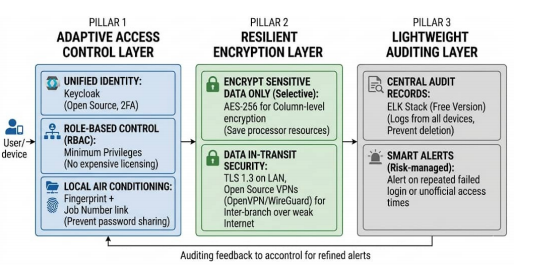
\includegraphics[width=0.85\textwidth]{1}
		\caption{Architectural Simulation of the Proposed Adaptive Framework}
		\label{fig:img_1}
	\end{figure}
	
	\section{Experimental Design and Protocol}
	The 'experimental design' for this study is primarily theoretical and analytical, focusing on the conceptual validation of the adaptive model rather than empirical experimentation. The 'protocol' involved a structured comparison of the proposed model's components against the baseline HIPAA technical safeguards and the NIST CSF, considering the unique constraints of the Yemeni healthcare environment. Table 3.1 details this comparative analysis and the resulting adaptive strategies.
	
	
	
	
	% مثال لإدراج جدول أكاديمي احترافي
	\begin{table}[H]
		\centering
		\caption{Comparative Analysis of HIPAA Technical Standards in the Yemeni Context}
		\label{tab:metrics}
		\begin{tabularx}{\textwidth}{lXXX}
			\toprule
			\textbf{HIPAA Standard} & \textbf{Technical Description} & \textbf{Importance in Yemeni Context} & \textbf{Adaptive Implementation Strategy} \\
			\midrule
			Access Control & Unique user IDs, emergency access, automatic logoff, encryption. & Critical for shared work environments with high personnel turnover \cite{abdulrab2021assessing}.&
			Break-the-glass protocols and local biometric (fingerprint) integration. \\
			Audit Controls & Recording and examining activity in ePHI systems. & Vital for accountability and incident investigation in fragile states \cite{al2023information}. &
			Leveraging existing system logs for real-time anomaly detection. \\
			Integrity &
			Protecting ePHI from unauthorized alteration or destruction.&
			Ensures accuracy of medical records for correct treatment decisions \cite{nist2024sp80066r2}. &
			Implementation of digital signatures and hashing for sensitive data columns. \\
			Authentication &
			Verifying the identity of the person or entity accessing ePHI. &
			Prevents identity impersonation in digital systems \cite{hasegawa2024cybersecurity}. &
			Multi-factor authentication (MFA) adapted for available local devices. \\
			Transmission Security &
			Protecting ePHI during transmission over networks. &
			Secures data exchange between departments and external parties \cite{saad2025fuzzy}. &
			Selective Encryption to minimize latency on legacy hardware. \\
			\bottomrule
		\end{tabularx}
	\end{table}
	
	The 'dependent variables' are the anticipated improvements in health data security posture, measured by the model's ability to enhance confidentiality, integrity, and availability of ePHI, reduce security gaps, and improve cyber risk management effectiveness. The protocol involves a qualitative assessment of how each adaptive component addresses these challenges, drawing upon insights from the comprehensive literature review and gap analysis. To ensure practical viability, the effectiveness of the proposed model is evaluated against a set of key performance indicators (KPIs) as detailed in Table 3.2.
	
	\begin{table}[H]
		\centering
		\caption{Evaluation Metrics for the Proposed Adaptive Model}
		\label{tab:metrics2}
		\begin{tabularx}{\textwidth}{lXXX}
			\toprule
			\textbf{Metric Category} & \textbf{Key Performance Indicators (KPIs)} & \textbf{Evaluation Method} & \textbf{Goal} \\
			\midrule
			Security Coverage & Percentage of HIPAA/NIST controls addressed.&
			Mapping Matrix Analysis & 
			$>90\%$ coverage of core technical safeguards. \\
			Resource Efficiency & CPU/Memory overhead of encryption \& auditing.&
			Simulated Load Testing & $<15\%$ performance impact on legacy systems. \\
			Operational Feasibility &
			Ease of use for non-technical medical staff. &
			Usability Heuristic Evaluation &
			High adoption rate with minimal training. 
			\\
			Risk Mitigation &
			Reduction in potential attack surface. &
			Threat Modeling (STRIDE) &
			Significant reduction in data breach probability. \\
			\bottomrule
		\end{tabularx}
	\end{table}
	
	\section{Baselines and State-of-the-Art Models}	
	The primary 'baselines' for comparison in this study are the standard HIPAA technical safeguards \cite{hhs2024hipaa} and the comprehensive NIST Cybersecurity Framework (NIST CSF) \cite{rahmany2026aida}. HIPAA provides stringent regulations for protecting ePHI, encompassing administrative, physical, and technical safeguards. The technical safeguards serve as a benchmark for secure access control, audit controls, data integrity, authentication, and transmission security. The NIST CSF offers a flexible framework for managing cybersecurity risk, structured around five core functions: Identify, Protect, Detect, Respond, and Recover.

	\renewcommand{\bibname}{References}
	\bibliography{ref}
	\bibliographystyle{ieeetr}
	
\end{document}